\subsubsection{University of Virginia} 
\paragraph*{Characterization of the large EIC GEM prototype with cosmic data:}\mbox{}\\
The initial tests of the large EIC GEM prototype showed  a significantly lower gain than the expected value of ~8000 when operating a typical triple-GEM with  Ar-CO2 (70/30) mixture at the nominal voltage 4100V. A likely explanation of the lower gain can be a problem during the production of the GEM foils at CERN with  the GEM holes sizes for the production batch slightly different from the standard GEM hole sizes, leading to a lower gain per GEM foil. In this case, even a relatively modest gain drop per GEM foil will lead to a significant gain drop in a triple GEM detector configuration. Increasing the voltage on the divider from 4100V to 4300V is enough to reach the nominal gain. However, due the large detector size and various challenges with stretching of the GEM foil during the assembly, we could not operate the detector in a stable way at 4300V. Therefore, we decided to use Ar-CO2 (80/20) mixture instead of Ar-CO2 (70/30) to be able to operate a typical gain of about 8000  at 4100V on the divider.\\
% 
\begin{figure}[htb]
\centering
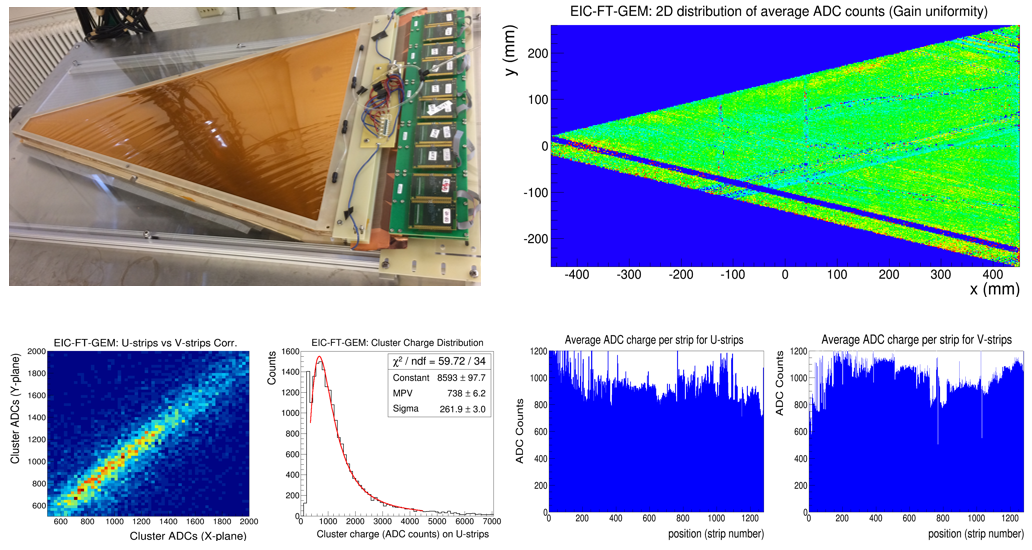
\includegraphics[width=1\columnwidth,trim={0pt 0mm 0pt 0mm},clip]{UVa_plots/eicCosmic}
\caption{\label{fig:eicCosmic}({\it Top left:}) EIC GEM prototype on the cosmic bench at UVa;  ({\it top right left:}) Gain uniformity: average charge (ADC counts) distribution over the active area; ({\it bottom from right to left:}) Charge sharing correlation between the top layer (U-strips) and bottom layer (V-strips); ADC charge distribution (ADC counts) on the top U-strips with the fit to Landau function;  Average charge (ADC counts) on  individual strip for U-strips and V-strips layers.}
\end{figure}
%
The prototype was characterized with cosmic for a three weeks period during which we collected 4M triggered cosmic events. Fig.~\ref{fig:eicCosmic} shows the detector on the cosmic bench in the Detector Lab at UVa and basic characteristics plots  from the data analysis. The plot on {\it top left:} shows a fairly uniform distribution of the average ADC per unit area (ratio of the total accumulated charge over the total number of hits inside the area)  across  the active area for 4 millions cosmic event. Efficiency drops caused by the spacers are clearly identified and we can also spot the effect of a broken strips. These results are a validation of  that the double-sided zebra connection scheme that we developed and tested on the prototype. However, the relatively wide dead area parallel to one side of the detector is very likely caused by connection between the zebra strips and the APV FE cards, outside the chamber. Excellent charge sharing  between the top layer (U-strips) and bottom layer (V-strips) of the U-V strips readout board  is shown on the charge correlation plot({\it bottom right:}) and is a validation of the improvement of  U-V readout design compared to the one that we tested in the first prototype developed in 2013 \cite{Gnanvo:2015xda}. The  charge distribution (in ADC channels) of the top layer strip ({\it bottom center:}) fit very nicely with the Landau function expected from the charge deposited by minimum ionizing particles. A good gain uniformity is also observed for the average ADC by each individual strips of the U and V strips layer respectively on the ({\it bottom center:}) and  ({\it bottom right:})  
%
%\paragraph*{Characterization of  $\mu$RWELL prototype with X-ray and $^{90}Sr$ sources:}\mbox{}\\
%We have completed the assembly of the meter-long low-mass Triple-GEM detector with \ang{30} stereo-angle U-V readout strip foil. The standard stretch-and-glue assembly technique was used for this prototype. Fig.~\ref{fig:uva_eic_gem_assembly} shows a couple of steps from this assembly process. The key points for the prototype relevant for EIC are:
%
%\begin{figure}[htb]
%\centering
%\includegraphics[width=1\columnwidth,trim={0pt 0mm 0pt 0mm},clip]{UVa_plots/uRwellXray}
%\caption{\label{fig:uRwellXray} ({\it Top left:}) Picture of the $\mu$RWELL structure on top of the 2D strip readout before final assembly. ({\it Top right:})  Cross section of $\mu$RWELL detector with 2D strip readout; ({\it Bottom left :}) Gain and efficiency curve ad a function of the electric field (E$_{Drift}$) in the drift; ({\it bottom center:}) Gain and efficiency curve as a function the electric field (E$_{{\mu}RWELL}$) in the  $\mu$RWELL structure; ({\it bottom right:}) Charge sharing correlation between the X-Y strips.}
%\end{figure}
%
\paragraph*{The prototypes in FTBF test beam at FNAL}\mbox{}\\
%
\begin{figure}[htb]
\centering
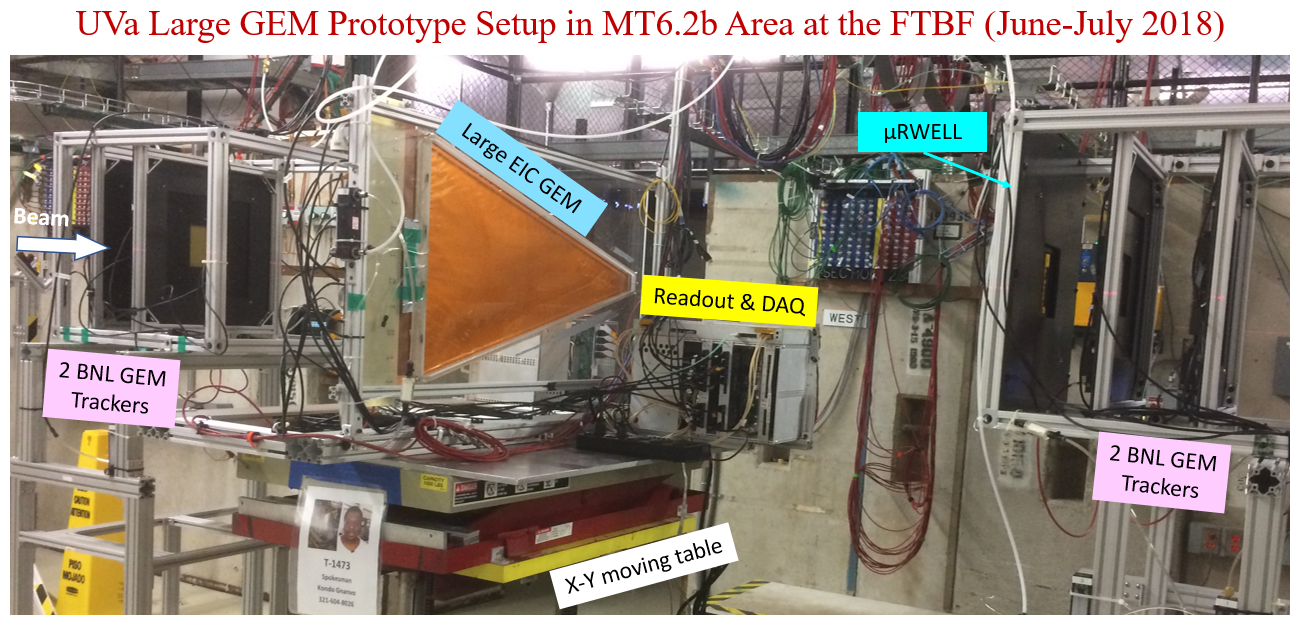
\includegraphics[width=1\columnwidth,trim={0pt 0mm 0pt 0mm},clip]{UVa_plots/ftbfSetup}
\caption{\label{fig:ftbfSetup} Setup of the large EIC GEM prototype on the moving X-Y table of MT6.2b area at the FTBF in June-July 2018, with two BNL GEMs for the upstream telescope and two other BNL GEMs combined our  small $\mu$RWELL prototype for the downstream telescope.}
\end{figure}
\begin{figure}[htb]
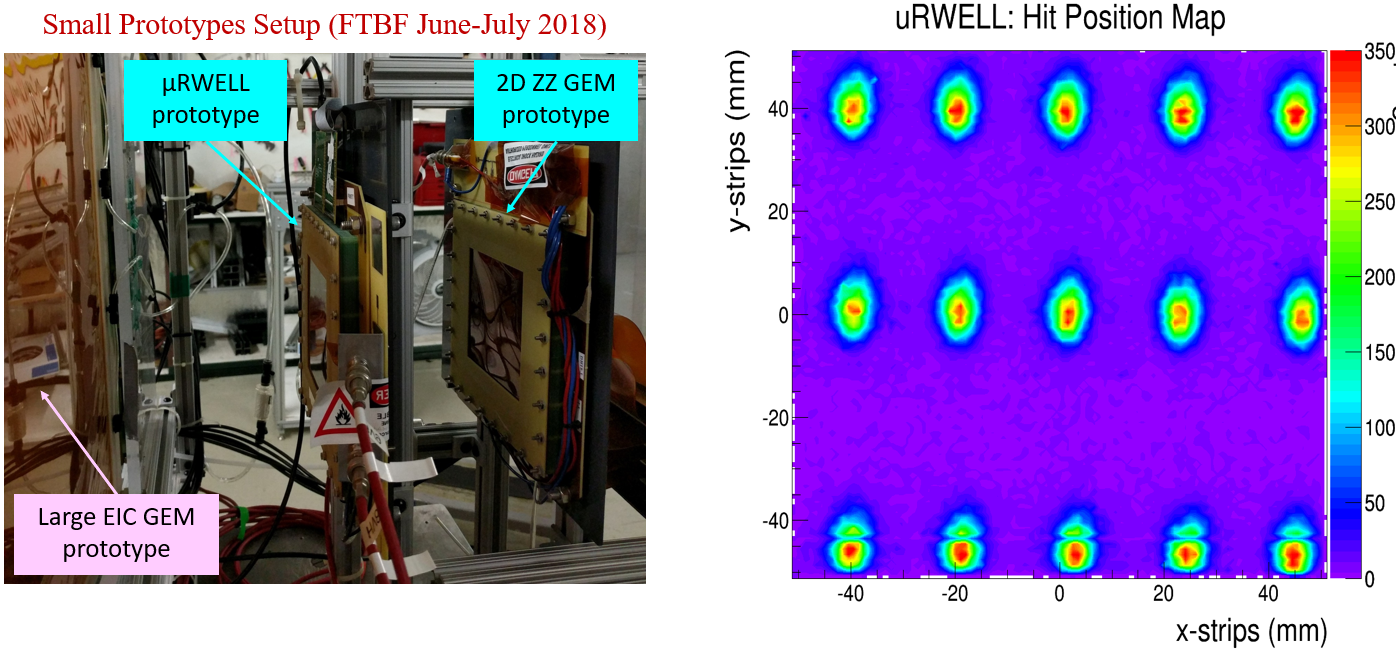
\includegraphics[width=1\columnwidth,trim={0pt 0mm 0pt 0mm},clip]{UVa_plots/ftbfSmallSetup}
\caption{\label{fig:ftbfSmallSetup} ({\it Left:}) The $\mu$RWELL prototype with 2D X-Y readout strip, the cross section of the detector is shown at the bottom; ({\it right:}) Setup of $\mu$RWELL  prototype and a small triple-GEM prototype with 2D zigzag strip readout at the FTBF in June-July 2018. The prototypes were installed on the same moving table behind the large EIC GEM.}
\end{figure}
%
The large EIC GEM prototype, the $\mu$RWELL prototype  and an additional small triple-GEM with 2D zigzag strip prototypes were brought to the Fermilab Test Beam Facility (FTBF) this summer (June 2018 - July 2018) for a period of 3 weeks and tested with the 120 GeV primary proton beam. The beam test campaign was a combined effort which includes M. Hohlmann's group  from Florida Tech (FIT), also testing  their large EIC GEM prototype with zigzag strip readout and K. Dehmelt and T. Hemmick's group from Stony Brook (SBU) testing their small TPC prototype with GEM readout. UVa and FIT shared the same large EIC GEMs setup with the prototypes installed on the X-Y moving table of the  MT6.2b area at the FTBF. For the tracking, our colleagues from BNL group provided four small triple-GEMs COMPASS readout. The setup is shown on  Fig.~\ref{fig:ftbfSetup}  with the four BNL GEMs and the $\mu$RWELL prototype used as upstream and downstream telescope. The detector configuration in the setup  was optimized to minimize the  multiple scattering impact on the resolution studies of the EIC GEM prototype. In addition, we also had a second detector configuration setup dedicated to a short study (one day beam time) of the small  $\mu$RWELL and the 2D zigzag GEM prototypes. In this second setup, the two small detectors were installed on the X-Y moving table behind the large EIC prototype as shown on Fig.~\ref{fig:ftbfSmallSetup}. All chambers, including the four BNL GEM trackers operated with the same Ar-CO2 (70/30) gas mixture and the same APV25-based Scalable Readout System (SRS) developed at CERN by the RD51 collaboration were used to read out all chambers. DATE and AMORE (developed by the CERN ALICE experiment) where used respectively as DAQ software and online/offline data analysis tool. The FTBF coincidence scintillators signal was used to trigger the DAQ at a rate of $\sim$ 400Hz.\\
%
\begin{figure}[htb]
\centering
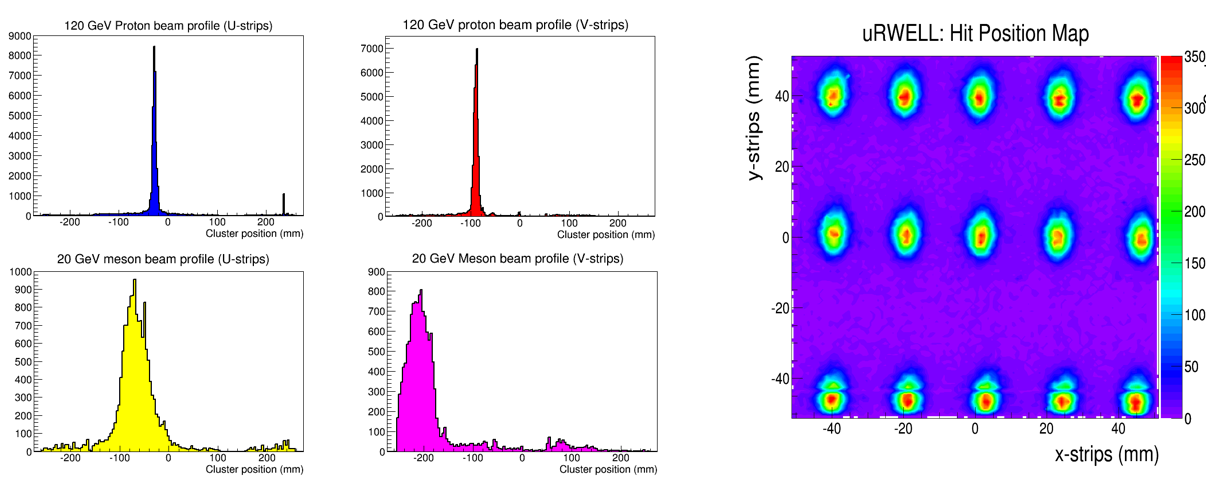
\includegraphics[width=1\columnwidth,trim={0pt 0mm 0pt 0mm},clip]{UVa_plots/ftbfBeamPosScan}
\caption{\label{fig:ftbfBeamPosScan} Beam profile reconstruction in the prototypes: ({\it Left and center}) 1D profiles of the 120 GeV Proton (top) and 20 GeV meson beam (bottom) in the EIC GEM top and bottom U-V strips readout layer. ({\it Right}) 2D reconstruction of 120 GeV proton beam from position scan in the $\mu$RWELL prototype.}
\end{figure}
%
Fig.~\ref{fig:ftbfBeamPosScan} shows a few example of the 120 GeV proton and 20 GeV meson beam reconstructed EIC GEM prototype as well as 2D proton beam reconstruction from a position scan run in $\mu$RWELL prototype. The horizontal line split for the spots at the bottom of the plots of the $\mu$RWELL are caused a few broken strips of the X-Y strips readout board.
%
\paragraph*{Production quality issues with the EIC U-V strips readout foil:}\mbox{}\\
\begin{figure}[htb]
\centering
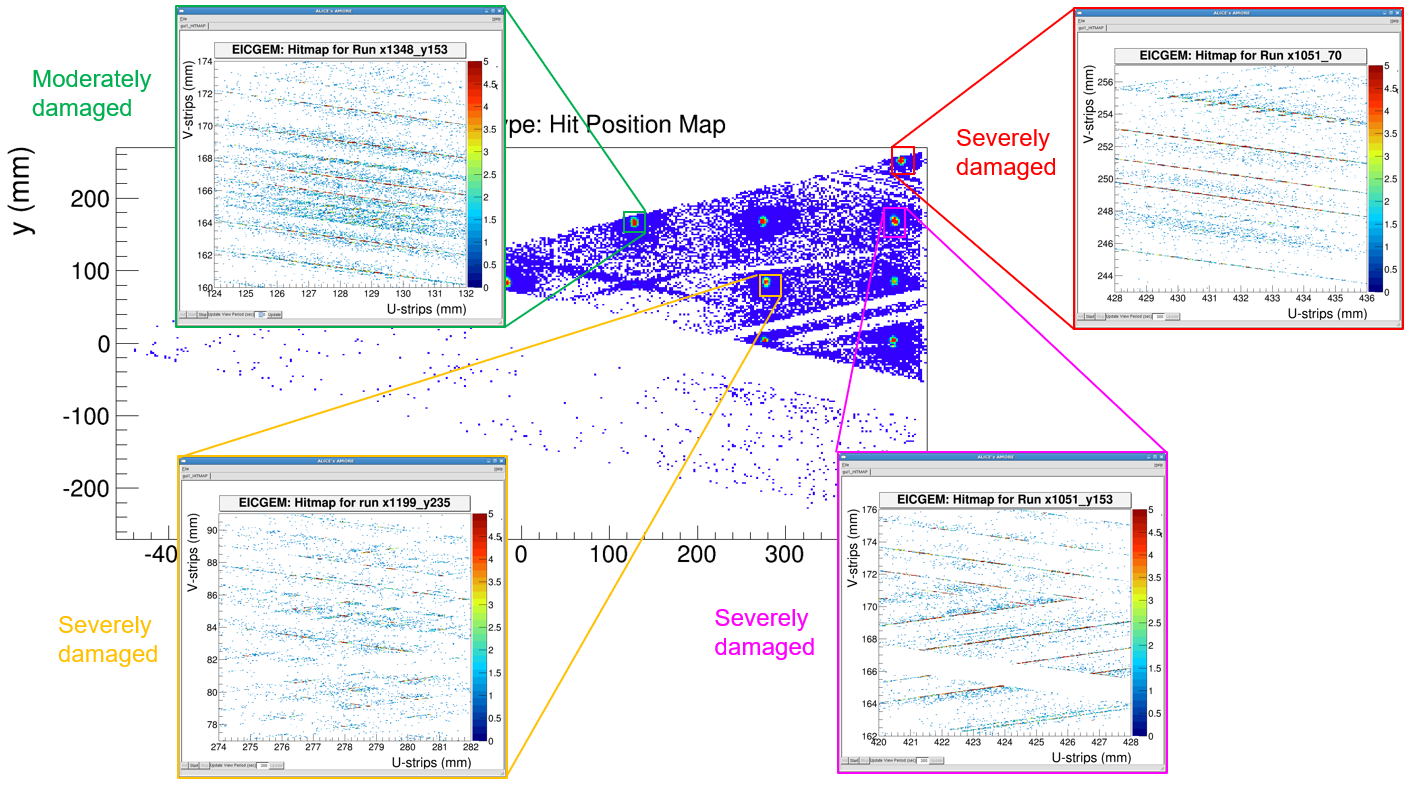
\includegraphics[width=1\columnwidth,trim={0pt 0mm 0pt 0mm},clip]{UVa_plots/eicPosScan}
\caption{\label{fig:eicPosScan}  2D  reconstruction of 120 GeV proton beam from position scan in the top half of the EIC GEM prototype. A zoom in of  reconstructed particle positions for four beam spots showing some unexpected patterns of non uniform distribution of the reconstructed particle positions.}
\end{figure}
Fig.~\ref{fig:eicPosScan} shows the 2D proton beam reconstruction from a position scan run in the large EIC GEM prototype. A zoom of the data plots reveals some unexpected patterns for reconstructed positions as shown for four location on the plots Fig.~\ref{fig:eicPosScan}. Instead of an uniform distribution, we actually observed on the plots that reconstructed positions are heavily concentrated around a set of discrete line parallel to the strips. This pattern suggests the possibility of a significant number shorts between the strips in both the top and bottom strip layers. A few consecutive shorted strips will results in identical large signal from the hit replicated on FE channels connected to these strips that would make it impossible to extract the  position information with good accuracy. The test beam data  seem to confirm that hypothesis. The problem seems more severe in some location than others as shown on the plots of Fig.~\ref{fig:eicPosScan}.  One possible source could be the double-sided zebra scheme connection that we developed and implemented for the large EIC prototype readout strips. Short contact could potentially also originate from the zebra strip or from the Panasonic-to-Zebra PCB interface that we use in these scheme. The investigation of origin of the bad data quality is ongoing.
%
\paragraph*{Track tit residuals analysis}\mbox{}\\
%
\begin{enumerate}
\item \textbf{Performances of BNL GEM trackers:}
%
\begin{figure}[htb]
\centering
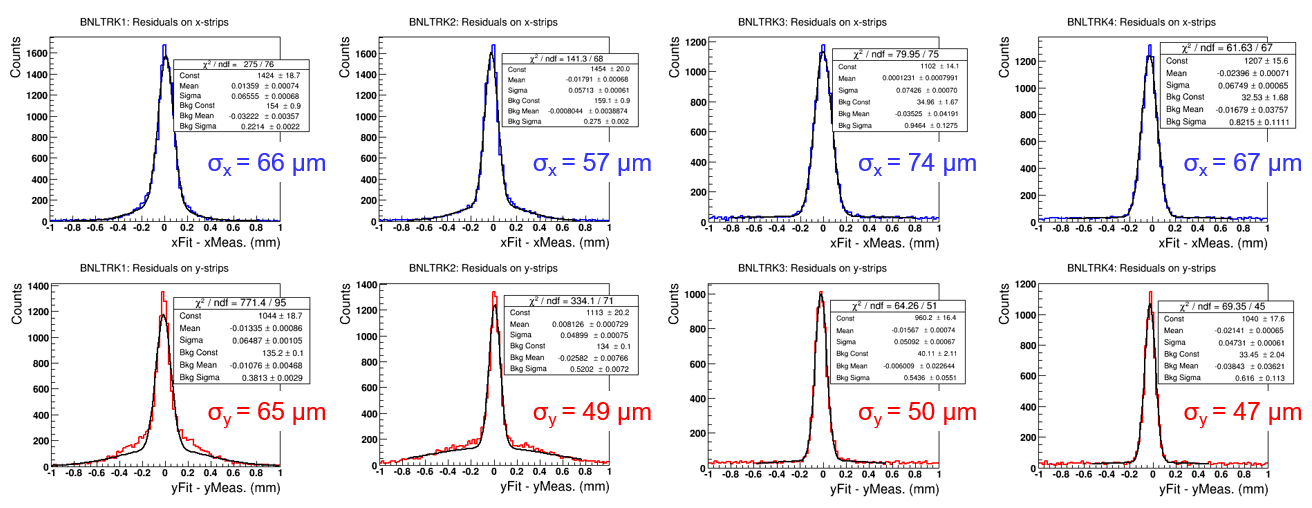
\includegraphics[width=1\columnwidth,trim={0pt 0mm 0pt 0mm},clip]{UVa_plots/trkResidual}
\caption{\label{fig:trkResidual} Residual distribution in x and y of BNL GEM trackers with the 120 GeV proton beam.}
\end{figure}
% https://www.overleaf.com/project/5bfc23f3c9ba6874cfc96bb5
\item \textbf{Large EIC GEM prototype:}
\begin{figure}[htb]
\centering
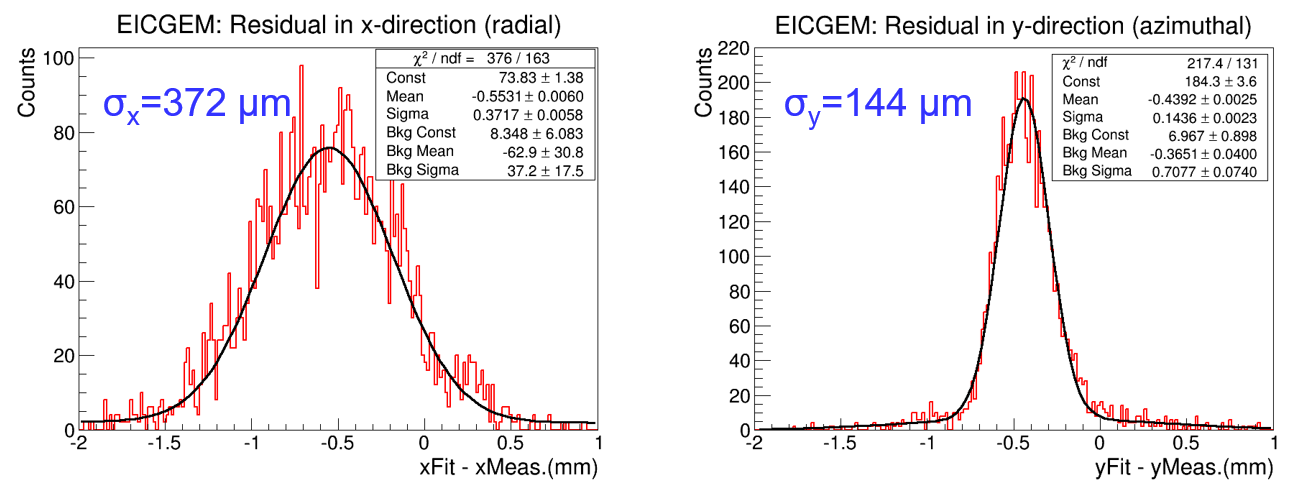
\includegraphics[width=1\columnwidth,trim={0pt 0mm 0pt 0mm},clip]{UVa_plots/eicResidual}
\caption{\label{fig:eicResidual} Residuals in x and y of the EIC GEM prototype with the 120 GeV FTBF proton beam.}
\end{figure}
%
We have completed the assembly of the meter-long low-mass Triple-GEM detector with \ang{30} stereo-angle U-V readout strip foil. The standard stretch-and-glue assembly technique was used for this prototype. Fig.~\ref{fig:uva_eic_gem_assembly} shows a couple of steps from this assembly process. The key points for the prototype relevant for EIC are:
%
\item \textbf{$\mu$RWELL prototype:}
%
For this Triple-GEM prototype, we use only foils including for the drift cathode and the U-V strips readout board, with no rigid PCB or support structure  in the active area. The 2D U-V strips readout layer and the drift cathode were all produced at CERN from the same copper clad Kapton base material used for the production of GEM foils.The elimination of rigid support structure in the active area of the detector is motivated by for low material requirement to minimize multiple scattering as well as photon induced background. Entrance and exit gas volume with 25 $\mu$m thick Kapton foil have been added to the stack of active foils for pressure balance inside the chamber in order to maintain uniform gap between different layers needed for an uniform gain across the active area.  Top left picture of Fig.~\ref{fig:uva_eic_gem_assembly} shows a cross section of the all foils EIC-FT-GEM prototype with the entrance and exit gas windows.
%
\begin{figure}[htb]
\centering
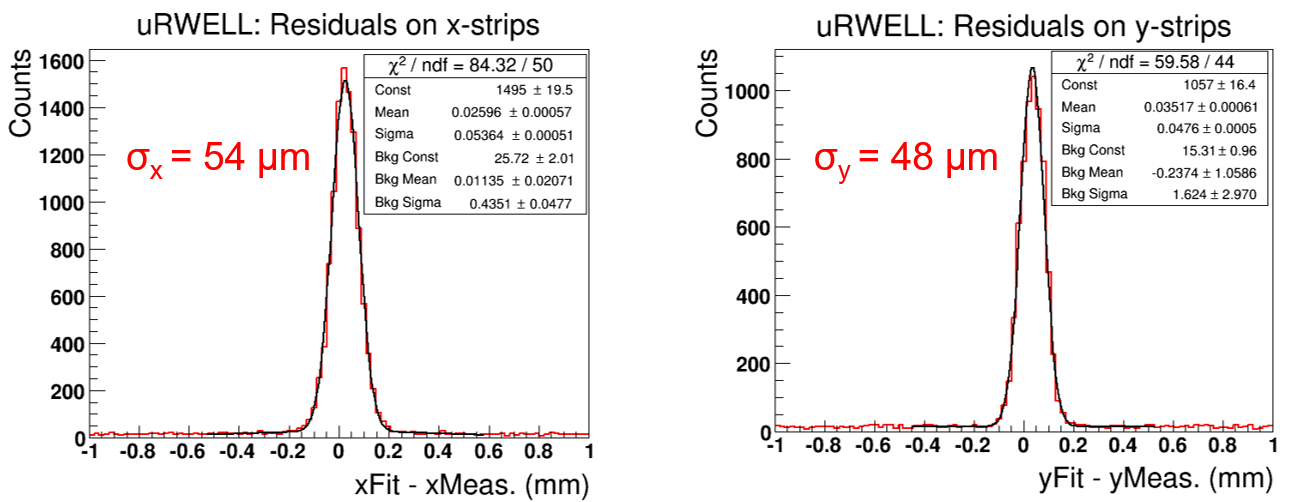
\includegraphics[width=1\columnwidth,trim={0pt 0mm 0pt 0mm},clip]{UVa_plots/uRwellResidual}
\caption{\label{fig:uRwellResidual} Residuals in x and y of the $\mu$RWELL prototype with the 120 GeV FTBF proton beam.}
\end{figure}
%
\end{enumerate}
